\begin{frame}{Súper Resolución}
    Bajo un enfoque \emph{clásico}, existen tres formas de mejorar la resolución 
    de una imagen:


    \begin{block}{Métodos}
        \begin{itemize}
            \item Amplificación de detalles existentes
            \item Suma de múltiples frames
            \item Único frame
        \end{itemize}
    \end{block}

\end{frame}

\begin{frame}{Predicción de resolución a partir de un único frame}
    ¿Cómo aumentar la densidad de pixeles de una imagen? 

    \pause
    \vspace{0.5cm}
    
    Predicción, aproximación... 
    
    \pause 

    \vspace{0.5cm}

    \begin{block}{Tipos}
        Dentro de las propuestas se encuentran los interpoladores:
        \begin{itemize}
            \item \emph{Adaptativos}: Algoritmos cambiantes por pixel
            \item \emph{No adaptativos}: Algoritmos estáticos a través de Algoritmos
            adyacentes. 
        \end{itemize}
    \end{block}

    Algunos de ellos incluyen algoritmos como \emph{vecino más cercano, bilineal, bicúbica,
    spline, entre otros.}
    
\end{frame}

\begin{frame}{Interpoladores no adaptativos}
    
    \begin{block}{Tipos}
        \begin{itemize}
            \item \textbf{Vecino más cercano} - Vecindad 1x1
            \item \textbf{Bilineal} - Vecindad 2x2 con promedios ponderados
            \item \textbf{Bicúbica} - Vecindad 4x4 con promedios ponderados 
        \end{itemize}
    \end{block}


    
    \begin{figure}[H]
        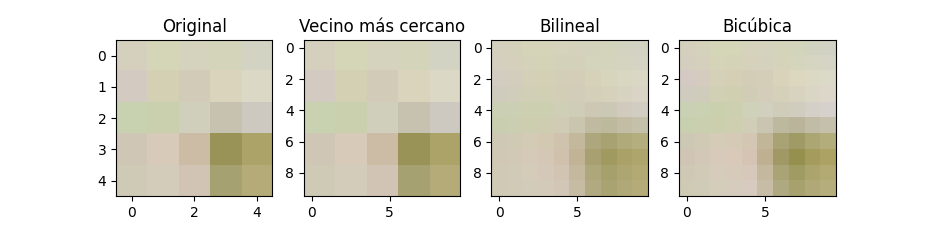
\includegraphics[scale = 0.45 ]{ tipos_interpoladores.png }
        \centering
        \caption{ Algoritmos de interpolación no adaptativos }
        \label{fig:interpoladores}
    \end{figure}

\end{frame}

\begin{frame}{Efectos de la interpolación}
    
    Todos los interpoladores no adaptativos intentan encontrar un equilibrio óptimo
    entre tres efectos no deseados: halos de borde, desenfoque y \emph{aliasing}. En la 
    Figura \ref{fig:efectos_inter} puede observarse el efecto para cada caso. 
    
    \begin{figure}[H]
        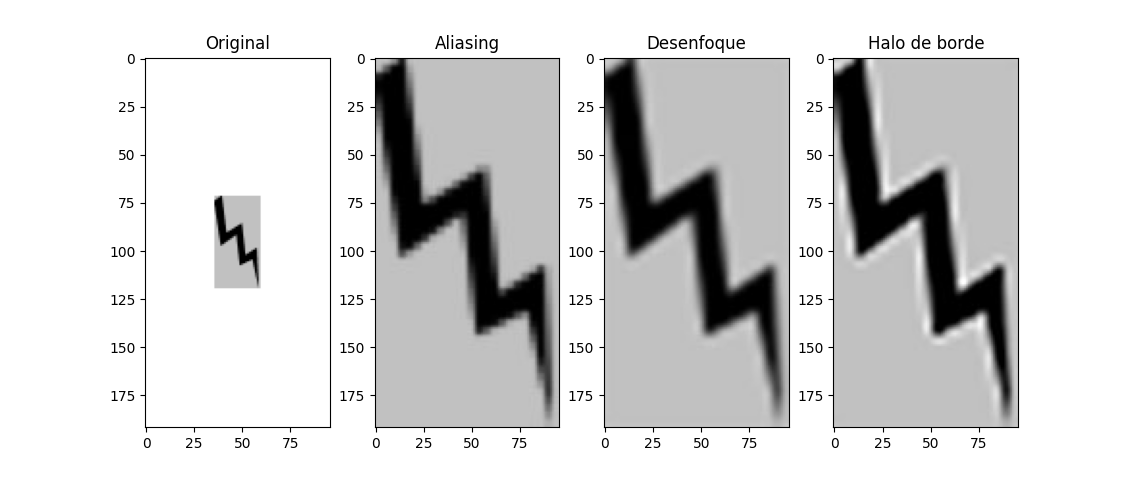
\includegraphics[scale = 0.35 ]{ efectos_inter.png }
        \centering
        \caption{ Efectos de interpolación}
        \label{fig:efectos_inter}
    \end{figure}

\end{frame}


\begin{frame}{Mejorar la interpolación de imágenes}
    
    \begin{block}{Dentro de las propuestas, \emph{Freeman et al} propone:}
        \begin{enumerate}
            \item La relación entre parches de alta y baja resolución
            es independiente del contraste de la imagen. 
            \item Los detalles están en las altas frecuencias 
        \end{enumerate}
    \end{block}

    \begin{figure}[H]
        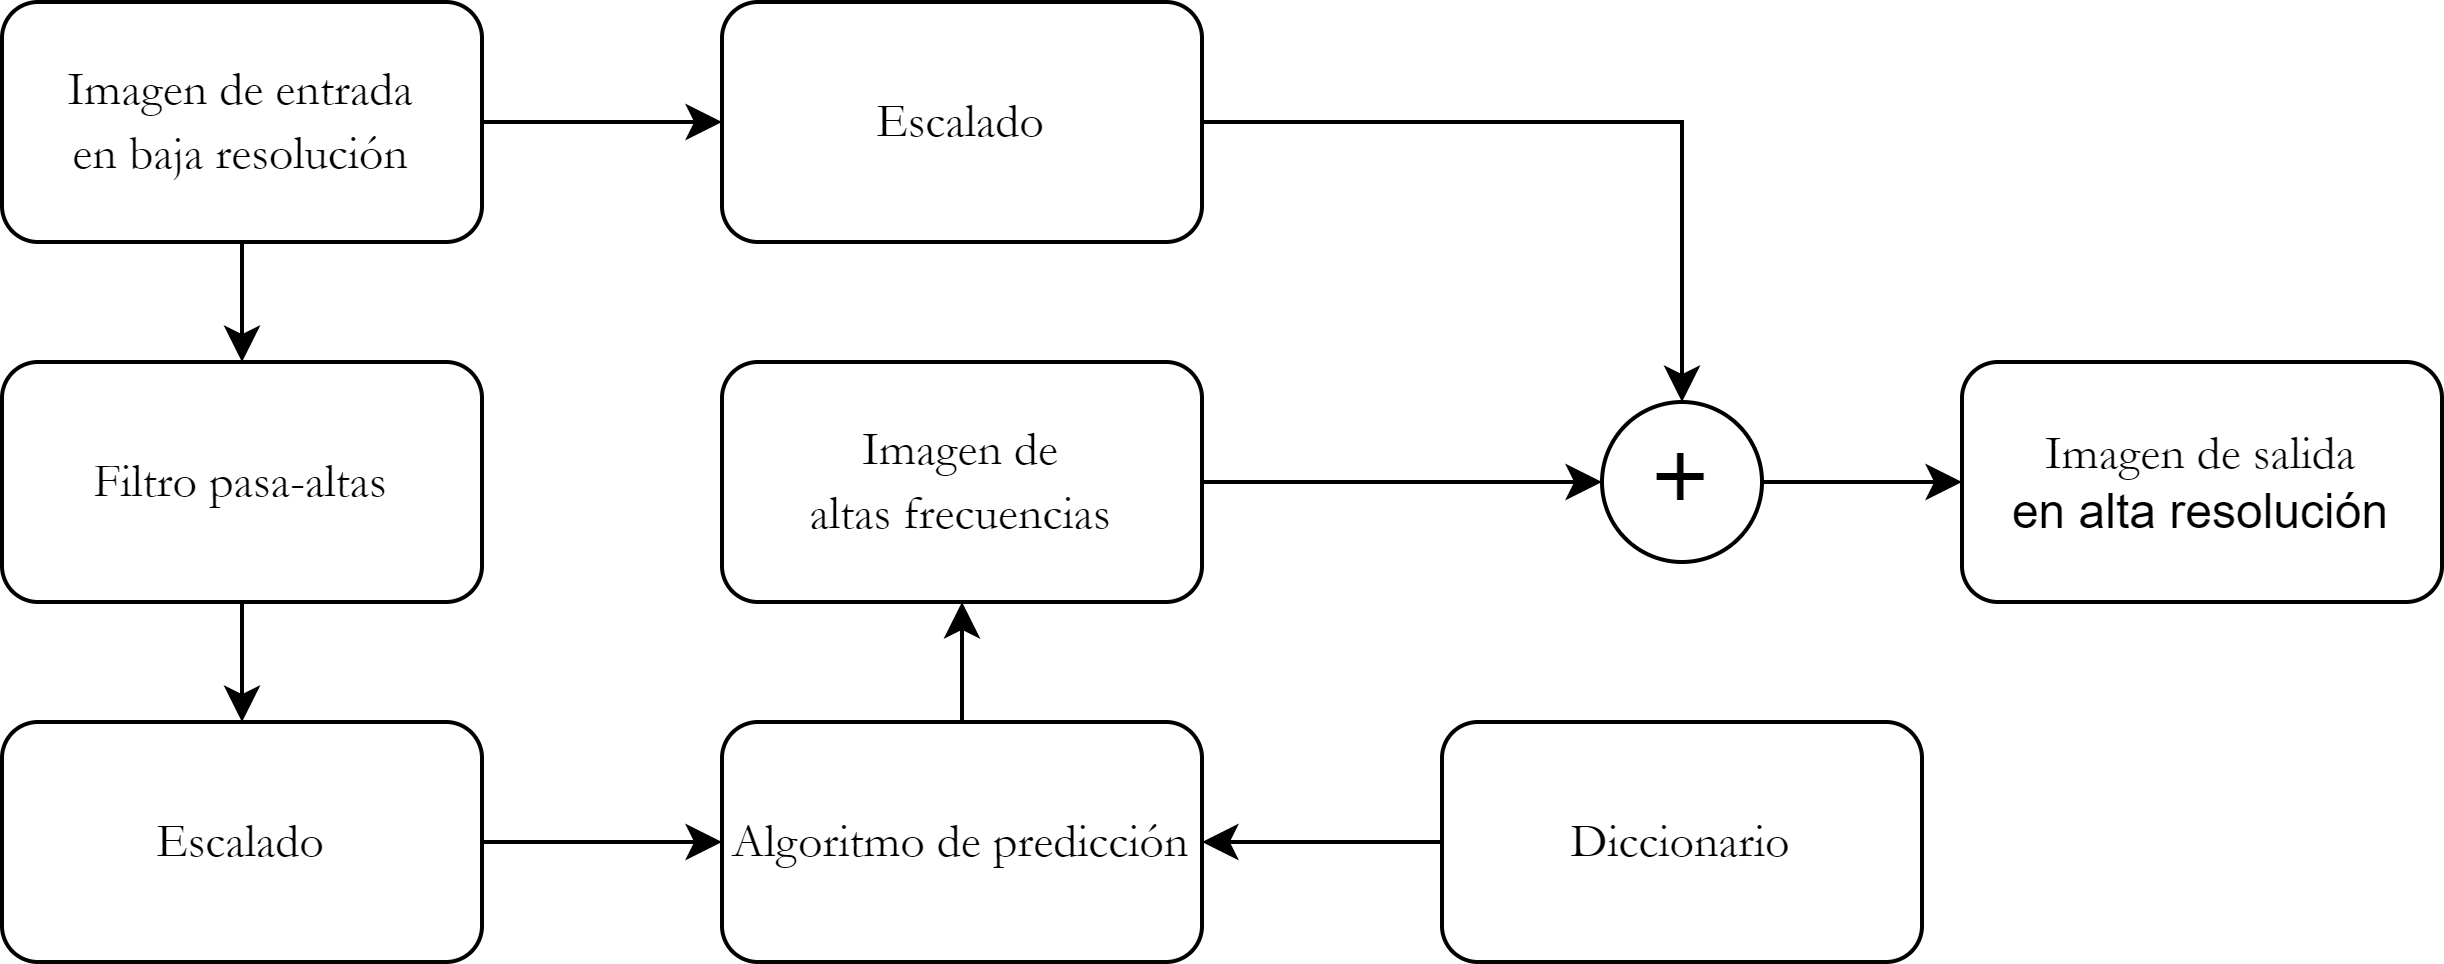
\includegraphics[scale = 0.4]{ fr_algoritmo.png }
        \centering
        \caption{ Algoritmo de súper resolución }
        \label{fig:fr_algoritmo}
    \end{figure}
    
\end{frame}

\begin{frame}{Diccionario}

    \begin{figure}[H]
        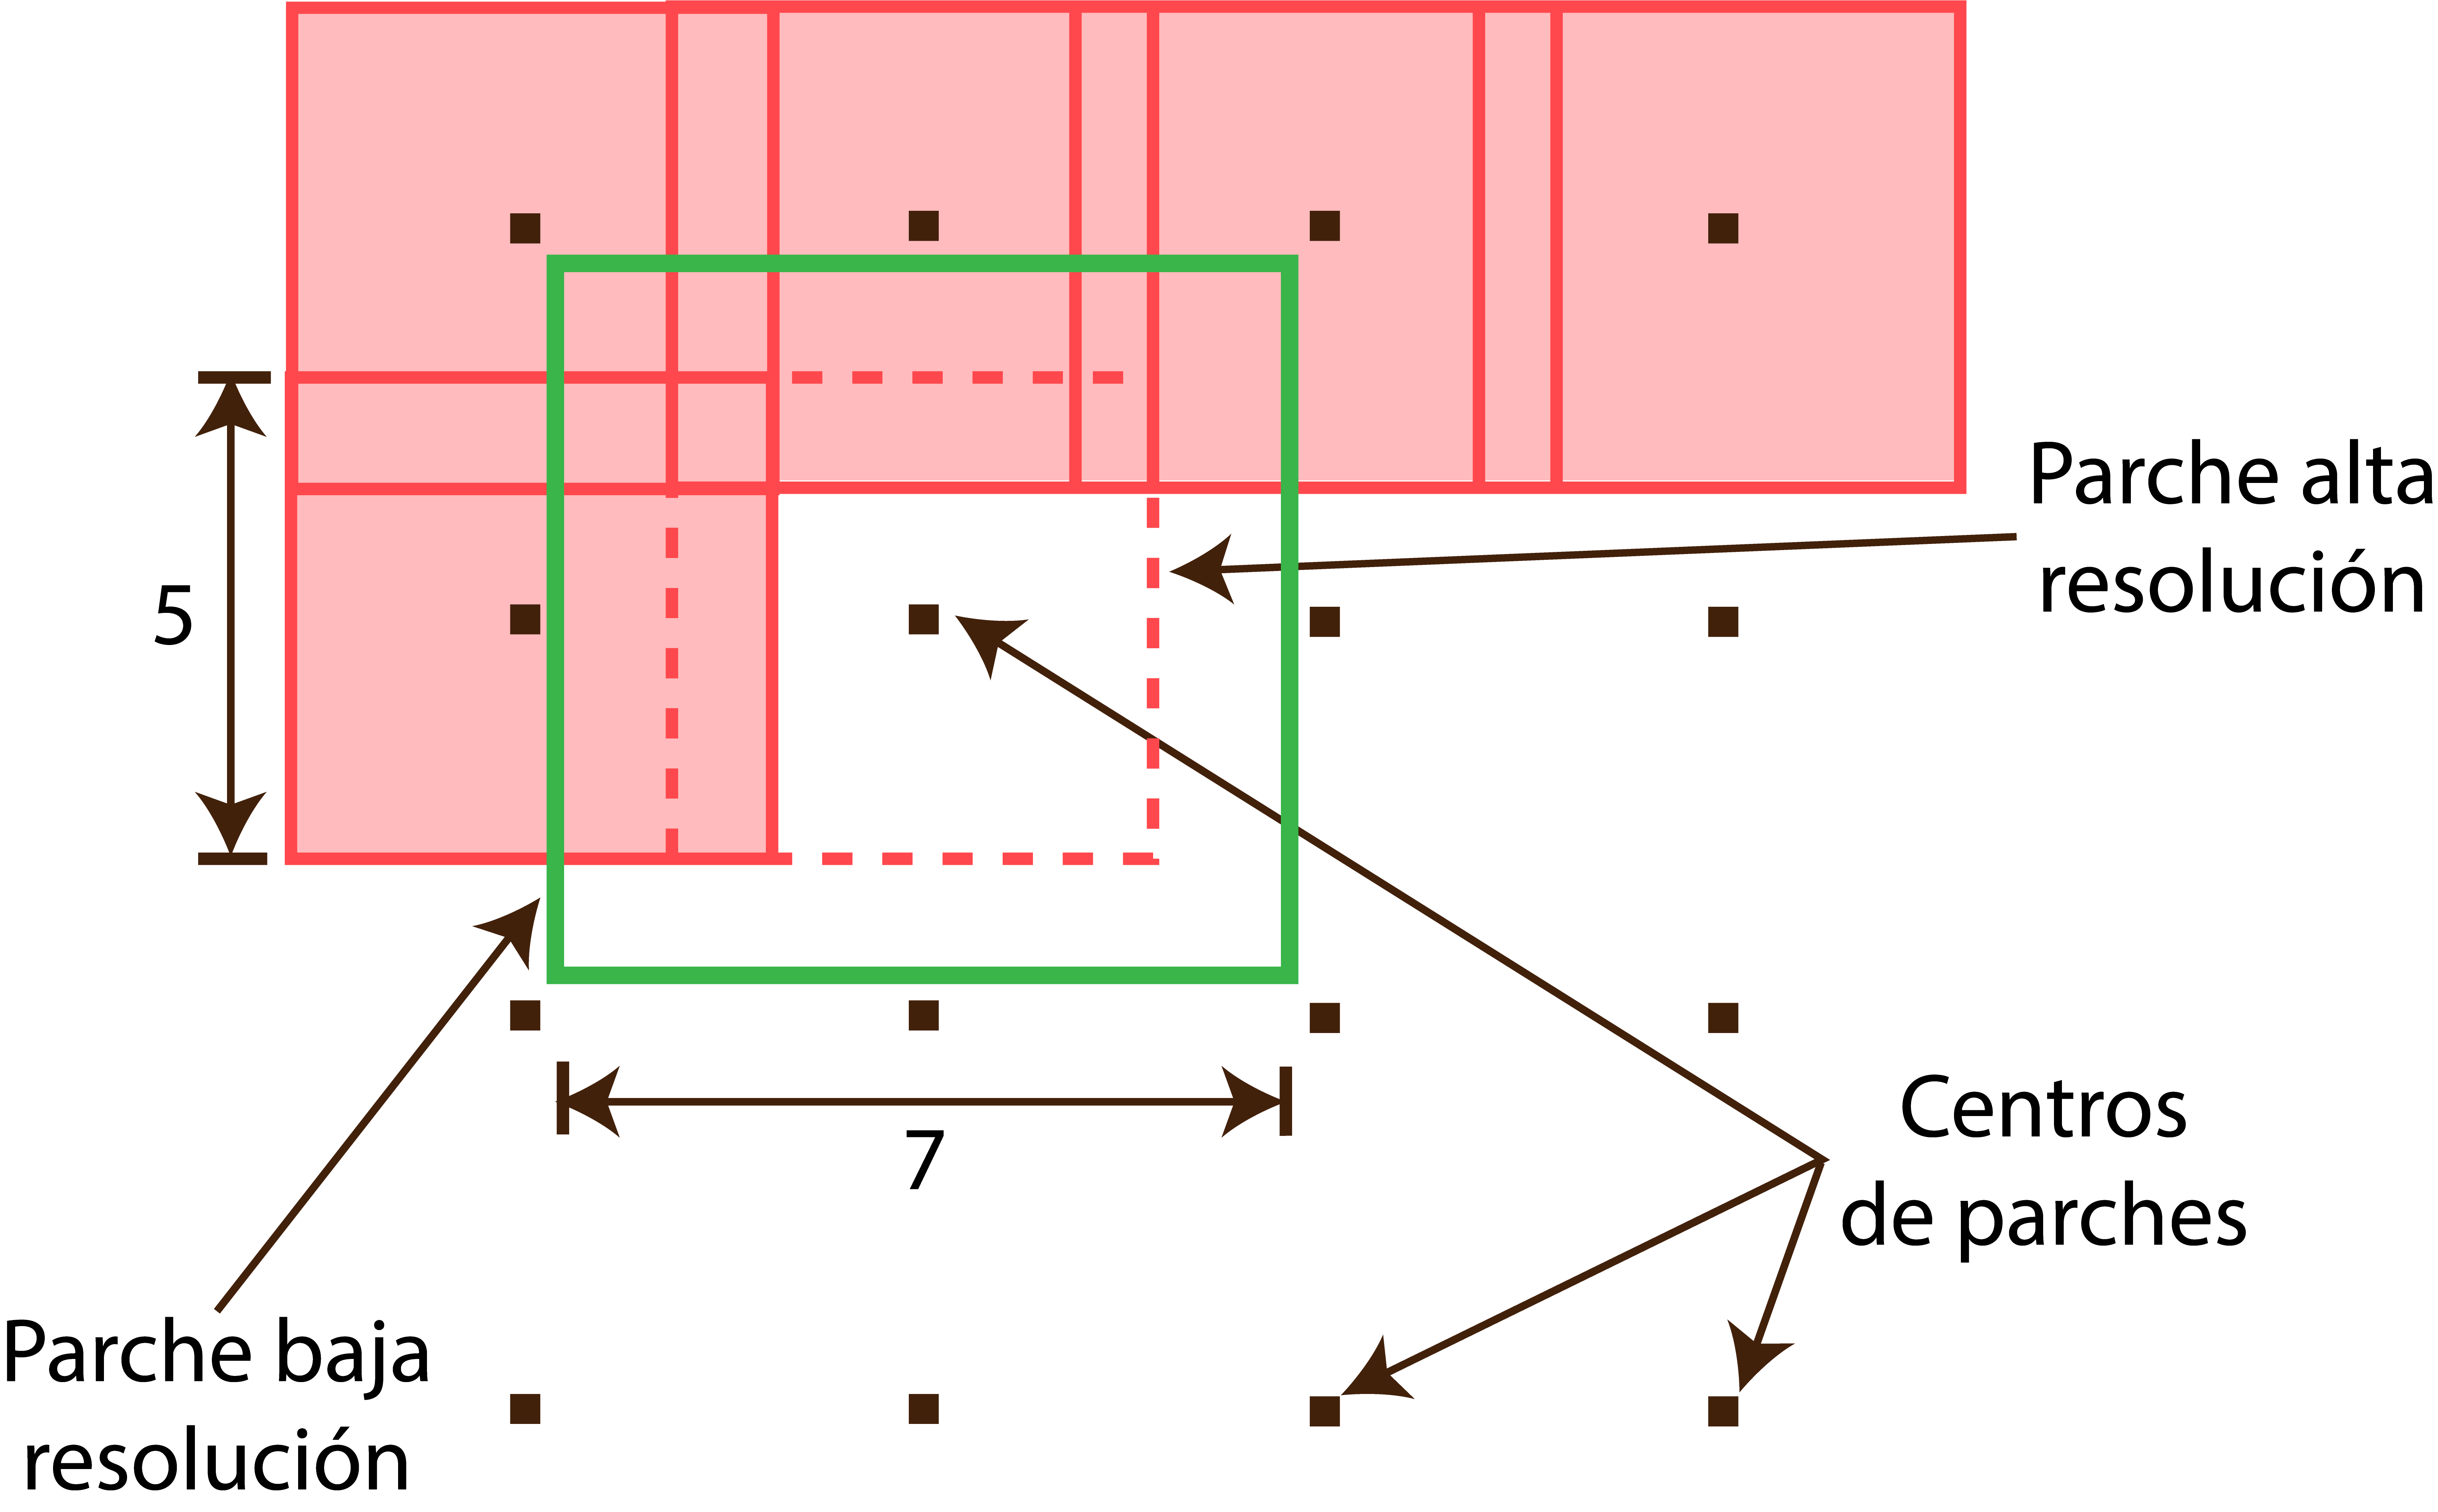
\includegraphics[scale = 0.18]{ fr_diccionario.png }
        \centering
        \caption{ Adquisición de parches de cada imagen}
        \label{fig:fr_dic}
    \end{figure}

    En específico, los parches de baja resolución deben reordenarse como un vector 
    en $\mathbb{R}^{1\times49}$ concatenado con la primera fila y primera columna
    del parche de alta resolución, resultando en un \textbf{vector para búsqueda} en $\mathbb{R}^{1\times59}$.
    
\end{frame}


\begin{frame}{Algoritmo de predicción}

    \begin{figure}[H]
        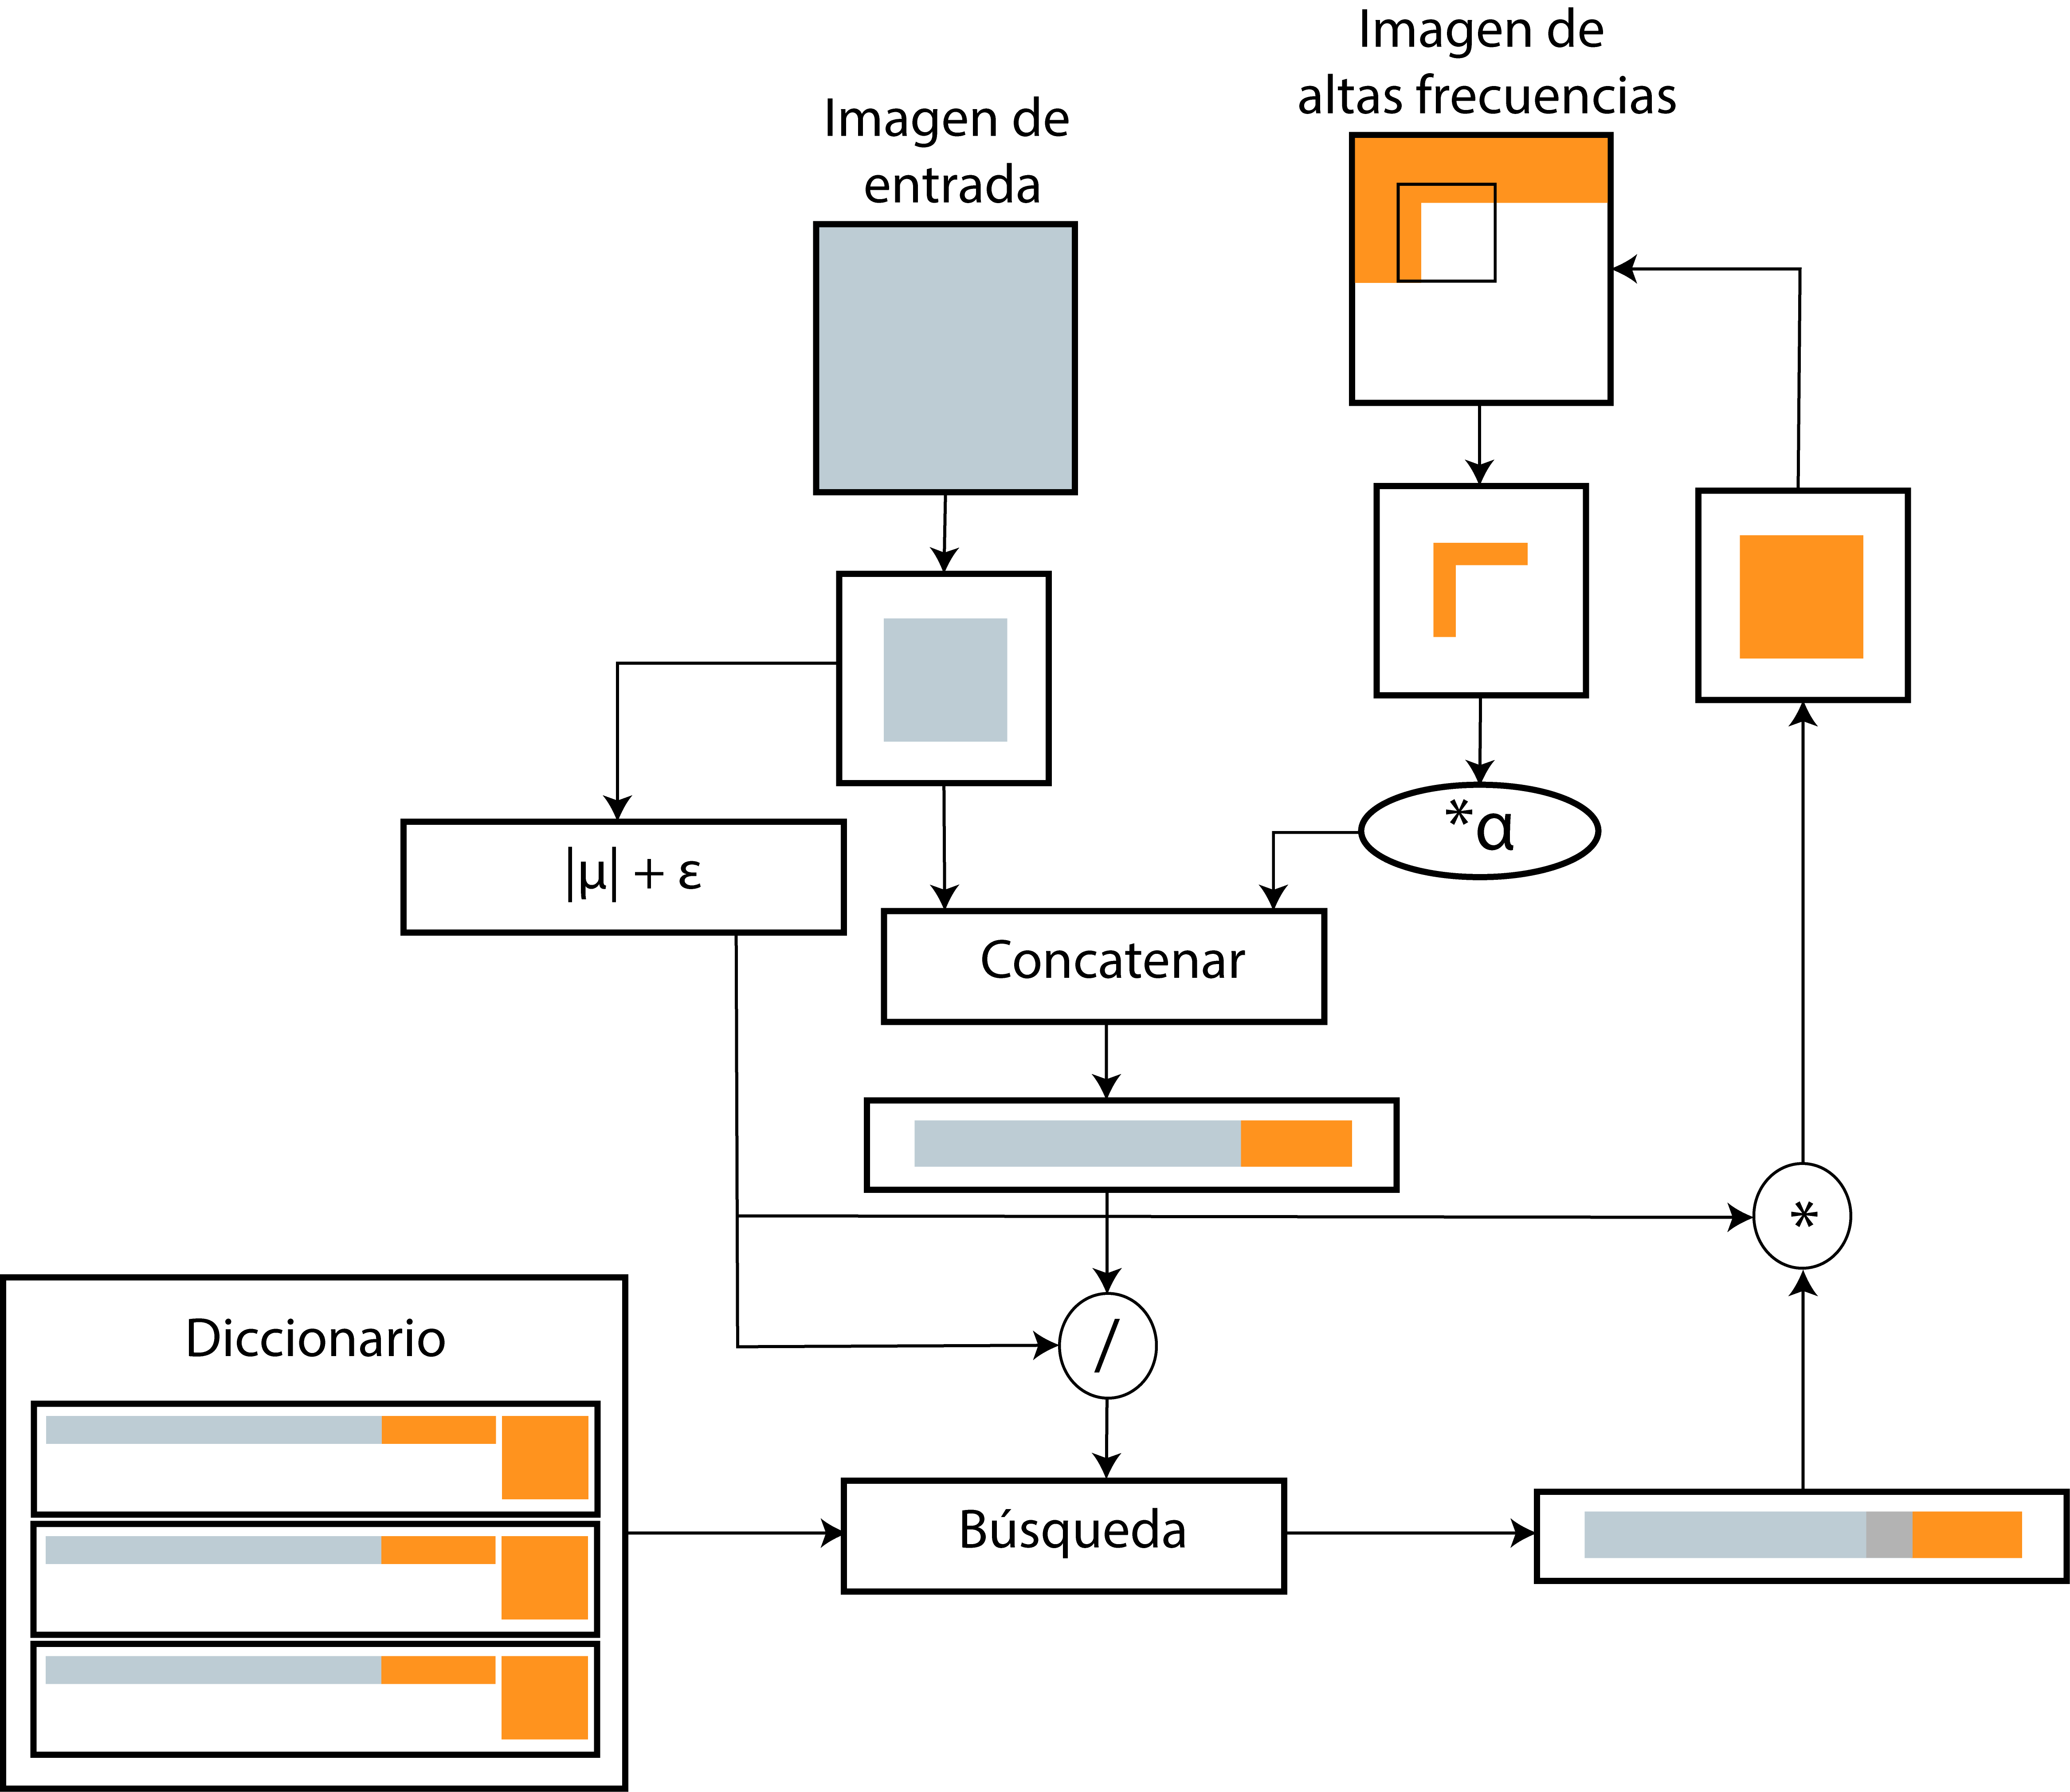
\includegraphics[scale = 0.3]{ freeman_prediccion.png}
        \centering
        \caption{ Algoritmo de predicción de imagen de frecuencias altas }
        \label{fig:fr_prediccion}
    \end{figure}

\end{frame}
